\chapter{PCA}
\section{Introduction}
Motivation: PCA is one of the most fundamental tools in data science and ML. Data is generally high dimensional. If it's higher than 3 dimensions you can't visualize it. If it's high dimensional, e.g., 100+ dimensions, then it can be inherently difficult to work with. Oversimplifying, this is because high dimensional space is so darn spacious, which causes fundamental objects like metrics to behave in counterintuitive ways. Though data may live in a high dimension, it's often the case that it's intrinsically lower dimensional. E.g., it lives on some lower dimensional manifold structure. If you can extract a reasonably ``faithful'' lower-dimensional representation of your data, then you can feed that to your algorithm instead of the raw data. Of course, the precise meaning of ``faithful'' here is complicated and depends on the use case, and is the basis for the entire field of dimensionality reduction. For our purposes, we'll consider using a linear map to take our data from a high dimension to a lower dimension. PCA will involve finding the ``best'' such linear map. 

TODO: Add a couple of motivating examples. Or links to some examples with nice pictures. 

Let $(x_i)_{i=1}^m$ represent some data set where $x_i \in \R^d$. We wish to represent the data in $n$ dimensions, for some $n<d$. More precisely, we wish to find the best linear transformation $T:\R^d\to\R^n$. The precise meaning of ``best'' is subjective. Typically, there are two notions of best considered. Both end up being equivalent, and allow one to derive PCA (meaning, find the map $T$) using fundamentally different mathematical tools. Each perspective can also allow one to contemplate different generalizations. (Double check this. But, for example, the minimum reconstruction error idea easily lends itself to an autoencoder type setup. Also, it's interesting to note that we could go from here to autoencoders. And then from autoencoders to VAEs. All of which give very different ways of thinking about things. Like, the objective you're trying to optimize is way different in a VAE.) We'll consider both approaches here. 

Before digging it, it is worth noting that, mechanically, PCA is quite simple. One simply computes the eigendecomposition of the sample covariance matrix 
\begin{equation} \label{S-def1}
S := \frac{1}{m}\sum_{i=1}^m x_ix_i^T.
\end{equation}
Recall that for a vector-valued random variable $x\in \R^n$, $Cov(X) := \E[(x- \mu)(x-\mu)^\T]$. WLOG (assuming finite mean) assume that $\mu=0$ to simplify notation. Elementwise, this has entries $(\E[x_ix_j])_{i,j=1,\ldots,n}$. 
Eigenvectors of $S$ with larger eigenvalues are considered more significant. Data is mapped to $n$ dimensions by projecting onto the span of the $n$ eigenvectors with largest eigenvalues. The focus of this discussion will be on understanding where this comes from and how to use it. 

The remainder of this document is organized as follows. We'll begin by deriving PCA from a variance maximization perspective and then from a minimum reconstruction error perspective. Then we'll consider kernel PCA. (Kernel PCA is a really nice way to start thinking about how kernels work, and solidify one's understanding of how PCA works. It's also useful as a nonlinear form of PCA that can allow one to, for example find clusters that might not be apparent by looking at linear mappings only.) Then we'll consider probabilistic PCA. 

\section{PCA: Maximum Variance Perspective}. 
Consider a data set (draw a 2d data set like an ellipse, not centered). Suppose you wanted to represent this using one dimension. How might you do it? We want to map these points to one dimension using a linear (or at least affine) map. The range of an affine map is a line in this space. Consider some different possibilities for a linear map. The most natural one is to draw a line through the mean of the data that goes along a direction of maximum ``variance.'' 

Let's extend this idea to our data set in $\R^d$. Without loss of generality, we assume that our data is centered so that $\sum_i x_i = 0$. Let\footnote{TODO: Make this notation consistent. Sometimes I treat $X$ as columnwise $x_i$}
$$
X = 
\begin{pmatrix}
 x_1^T\\
 \vdots\\
 x_m^T
\end{pmatrix}
\in \R^{m\times d}. 
$$
Let 
$$
S = X^T X \in \R^{d\times d},
$$
denote the sample covariance. Note that this agrees with the definition in \eqref{S-def1}. This can be seen by thinking of multiplication blockwise with components $x_i$. In my experience, $S$ is sometimes referred to as the covariance matrix. This is misleading since there are no probability distributions here. However, $S$ may be thought of as an estimator of the covariance matrix. Here, we'll call $S$ the sample covariance. 

We will begin by considering a projection onto a one dimensional subspace that maximizes the variance. Of course, a true probabilistic notion of variance is not defined here. Our goal is the following
\begin{align} \label{maxvar_opt_prob}
\max_{d\in R^n} ~& \sum_i (x_i^\T d)^2\\
\mbox{s.t.}~ & \|d\| = 1.
\end{align}
Note that the objective function may be thought of as the sample variance of the projected data. The projected data has zero mean, because we assumed the original data has zero mean, and a linear operation (projection) does not change this.\footnote{Getting an unbiased estimator of the variance is a little tricky. Usually, you use $\frac{1}{m-1}\sum_i (x_i - \bar x)^2$, where $\bar x$ is the sample mean. But if the sample mean is known, like here, you can plug it in directly and scale by $1/m$. However, here, we ignore the scaling, because it's not relevant to the optimization problem. TODO: Double check this.}


\subsection{Digression: Lagrange Multipliers}
Before solving this problem, we take a brief digression to discuss Lagrange multipliers.
In modern usage, this is usually wrapped up into the KKT conditions. Here, we will do something slightly different. 
Consider an optimization problem of the form
\begin{align} \label{eq:opt1}
\min_{x\in \R^d}~   & f(x)\\
\mbox{s.t.} ~ & h(x) = 0
\end{align}
where $h(x)$ is differentiable (do we need $C^1$?). 
Define 
$$
L(x, \lambda) := f(x) + \lambda h(x)
$$
to be the Lagrangian. The variable $\lambda$ is often referred to as a Lagrange multiplier. 

\textbf{Claim}: A solution of \eqref{eq:opt1} must satisfy $D L(x,\lambda) = 0$, where $D$ denotes the derivative w.r.t both variables.

The rest of this section discusses proving that result, but can be skipped if you're willing to take it on faith. The claim follows readily from the following Lemma:
\begin{lemma}
Suppose $g: \R^n\to \R$ is differentiable (Do I need $C^1$? This will probably pop out of the IFT usage.) and let $S := \{g(x) = 0\}$. For $x\in S$, if $v$ is a tangent vector to $S$ at $x$ then $v^T \nabla g(x) = 0$. 
\end{lemma}
If you have a solution $x^*$ to \eqref{eq:opt1}, then $x^*$ should satisfy the constraint, and $\nabla f(x^*)$ should be orthogonal to the constraint set (meaning, orthogonal to the tangent plane at $x^*$). If this were not true, then you could find another point in the constraint set that's slightly better by following the gradient. (How to formalize this?) However, by the preceding lemma, the condition that the gradient is orthogonal to the constraint set is the same as saying the that $\nabla f(x^*)$ and $\nabla h(x^*)$ are collinear, i.e., $\nabla f(x) = \lambda h(x)$ for some $\lambda$. If you have multiple constraints, then you must have $\nabla f(x^)$ orthogonal to the tangent plane of the intersection. This is a smaller set. The condition changes to $\nabla f(x^*)$ must be a linear combination of the constraint gradients. i.e., $\nabla f(x) - \sum_i h_i(x) = 0$. Intuitively, what we're stating here is that $\nabla f(x)$ has a little more freedom. As long as it doesn't have a component in the intersection of the two tangent planes, you're OK. The intuition becomes clear when you have a 1d space curve embedded in 3d. Or just use an example with a plane and a line. With the planar constraint, you need the gradient to be collinear with the normal vector. When you intersect with another planar constraint, then you get a little more flexibility in where the gradient of $f$ can point. 

The intuition for this is that if the gradient were not orthogonal to the tangent plane (or whatever kind of set) of the level set, then it couldn't actually be a level set. Think of a 2d example, The function would change slightly going in the direction in $S$ where the inner product with the gradient is nonzero. There is probably a proof that you could follow this way. A standard, and slicker proof is the following. Consider $x(t)$ to be any parameterized curve lying $S$. We have $g(x(t)) = 0$. Differentiating and applying the chain rule we see that 
$$
\nabla g(x(t)) \dot x(t) = 0.
$$ 
By construction, $x(t)$ is always tangent to $S$. Hence, this proves the result. 

Of course, this is a glib and incomplete proof. How do we actually know such an $x(t)$ exists, and how do we construct one? The right tool for this is the implicit function theorem. Consider: If $\nabla g(x) =0$, then there is nothing to show. If $\nabla g(x) \not = 0$, then there exists some variable in which it is nonzero. WLOG, let this be the last element. The implicit function theorem allows us to construct a mapping from a subset of variables to another subset of variables if the appropriate component of the determinant is nonsingular. In this case, we can construct a mapping from the coordinates $(x_1,\ldots, x_{n-1})$ to $x_n$ that keeps us in the set. That is, there exists a $C^1$ function $h:\R^{n-1}\to\R$ such that
$$
g(x^{n-1}, h(x^{n-1})) = 0,
$$
in some neighborhood of $x$, where I've used the shorthand $x^{n-1} = (x_1,\ldots,x_{n-1})$. Now, let
$$
r_i(t) := (x_1,\ldots, x_{i-1}, t, x_{i+1},\ldots, x_{n-1}, h(x_1,\ldots, x_{i-1}, t, x_{i+1},\ldots, x_{n-1})), \quad i=1,\ldots, n-1.
$$
These are $n-1$ curves that are contained in $S$ and pass through $x$. Moreover, their tangent vectors are linearly independent at $x$ (right)? The chain rule argument shows that the gradient is orthogonal to each. From this, we conclude that it is orthogonal to each linear combination, and hence orthogonal to the tangent space. 

IMPORTANT NOTE: Do we know that the tangent space is $n-1$ dimensional? Is this like a proof that that holds whenever the gradient is nonzero? Can the level set only be lower dimensional on sets where the gradient is zero? Yes. If the gradient is nonzero, then the gradient defines the normal vector to a plane. You should be able to argue that moving in any direction in that plane should hold things constant. I mean, really, you just apply the IFT to make that rigorous. 

\subsection{Return from digression}
Note that 
$$
 \sum_i (x_i^\T d)^2 = \sum_i d^\T x_i x_i^\T d = d^\T \left( \sum_i x_i x_i^T\right) d = d^T S d.
$$
Hence, computing the Lagrangian of \eqref{maxvar_opt_prob} we have
$$
L(d, \lambda) = d^\T S d + \lambda (\|d\|^2 - 1)
$$
and so
$$
L(x,\lambda) = 
\begin{pmatrix}
2Sd - 2\lambda d\\
\|d\|^2 - 1
\end{pmatrix}.
$$
Setting the derivative to zero we see that solutions to \eqref{maxvar_opt_prob} must satisfy
\begin{align}
Sd & = \lambda d\\
\|d\|^2 & = 1
\end{align}
These are exactly the eigenvectors/values of $S$. Out of this set, the eigenvector with largest eigenvalue optimizes \eqref{maxvar_opt_prob}. 

It's worth noting that the other eigenvalues are stationary points of \eqref{maxvar_opt_prob}. The stationary points of the Lagrangian find all points where the gradient of $f$ is orthogonal to the tangent space of the constraint. This seems a bit counterintuitive, since the objective in \eqref{maxvar_opt_prob} is convex. However, an example illustrates the point. 

Consider a 2d example: $f(x) = x^T A x$ where $A = diag(1, 2)$. Clearly, this is a parabaloid. Constrained to the unit ball, this problem is nonconvex. It has a local maximum along one of the axes and a local minimum along another. This is illustrated (poorly) in Figure \ref{fig:constrained-eig-opt}. In general, the intersection of the unit ball and eigenvectors will give you local maxima/minima of this problem. 

\begin{figure}[h] \label{fig:constrained-eig-opt}
\centering
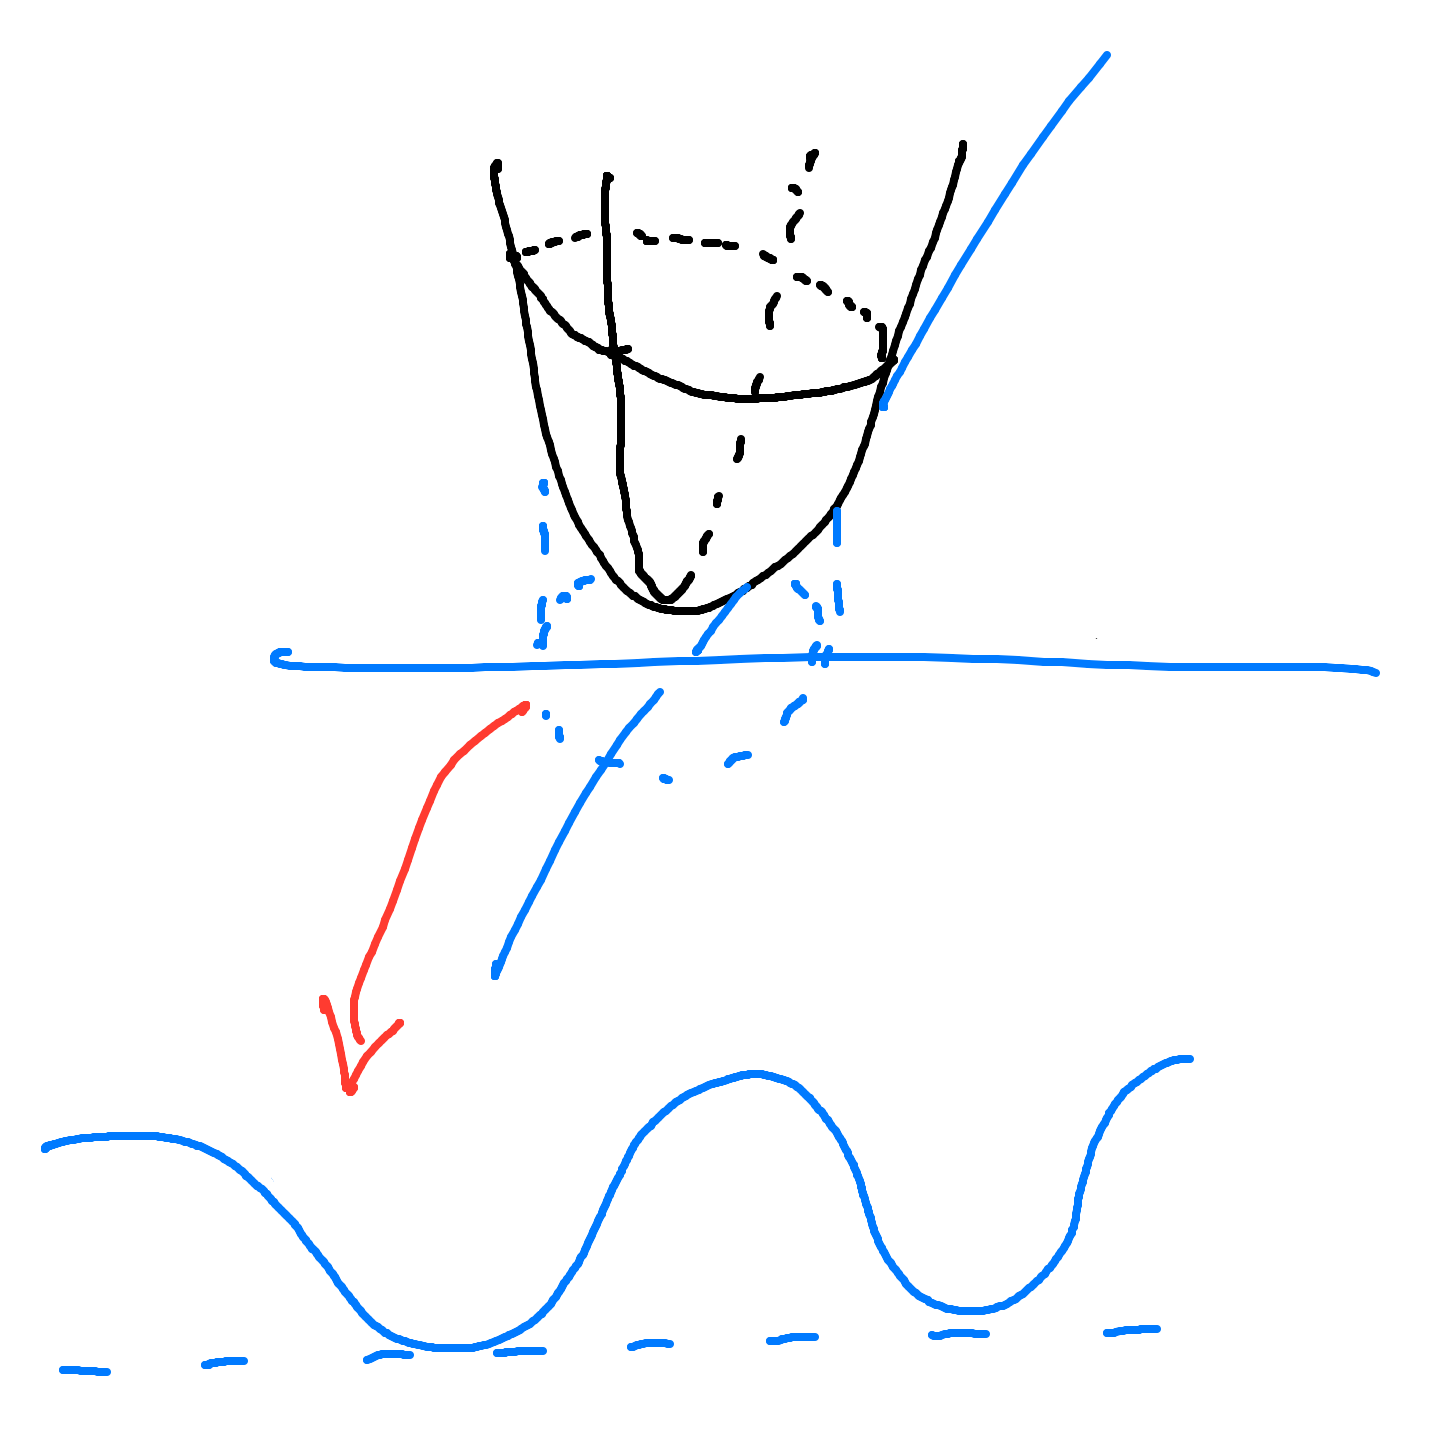
\includegraphics[width=10cm]{figs/PCA/Constrained-opt-eig.png}
\caption{Illustration of constrained optimization problem. The objective is a parabaloid constrained to the unit sphere. The parabaloid should look less symmetrical, but my drawing skills aren't great. Below, the unit sphere is unwrapped and the constrained objective is shown.}
\end{figure}

TODO: Connect this to the variational characterization of eigenvalues? 

Thus, if $n = 1$, we have found the subspace that provides maximal variance. For $n>1$, a similar technique can be used via an inductive argument. We won't follow the inductive argument through all the way here, but the idea is the following:

1. If you have an $r-1$ dimensional space of maximal variance, and you want to find the $r$, you subtract out the directions you've already found. (Draw a 2d picture for this.) Let
$$
\tilde X = X - \sum_{i=1}^{r-1} d_i d_i^\T X
$$
Here, we project $X$ onto each of the directions we've already found and subtract this from our dataset. (NOTE: Make sure $X$ contains $x_i$ as column vectors, otherwise need to use the transpose.) 
Let 
$$
\tilde S = \tilde X\tilde X^\T. 
$$
This is the sample covariance of the new data. Optimizing $\max_d^\T \tilde S d$ will give us the next direction of maximal variance. One may confirm that the eigenvalues of $\tilde S$ are the $d-r$th largest eigenvalues of $S$. (The larger eigenvalues, corresponding to directions we subtracted out are zero.) This is confirmed by expanding $\tilde X$ in the definition of $\tilde S$ and confirming that smaller eigenvalues of $S$ are eigenvalues of $\tilde S$. We see that the largest eigenvalues of $\tilde S$ gives us the next direction of maximal variance. 

TODO: What's missing from this proof is the inductive step. If we've found $d_{n-1}$, then how do I show that this really gives us the 2d subspace with optimal variance? 

\section{PCA: Minimum Reconstruction Loss Perspective}
TODO: Copy in other notes

\section{Interpreting PCA}
 In PCA, one can consider the latent codes or the projection to a lower dimensional subspace. The former can be thought of as a dimensionality reduction technique, while the latter may be thought of as a compression technique. 

To apply PCA, we choose some $r$ representing the number of principal components we wish to retain. Let $(v_i, \lambda_i)_{i=1}^r$ denote the $r$ largest eigenvalues/vectors, $v_i\in \R^d$. 
A data point, either from the training set, or a new point, is projected onto the principal components via
\begin{equation} \label{eq:PCA-proj}
\sum_{i=1}^r v_i v_i^\T z = \underbrace{(v_1,\ldots, v_r)}_{=: V} 
\begin{pmatrix}
v_1^\T\\
\vdots\\
v_r^\T
\end{pmatrix} z = \underbrace{V V^\T}_{=: P} z
\end{equation}
where $z\in \R^d$ is the point we wish to project. Note that $P: \R^d\to\R^d$. The projection $P$ takes data from $\R^d$ and embeds it onto a lower dimensional subspace in $\R^d$. The dimension of the subspace and the rank of $P$ are both $r$. This is illustrated in Figure \ref{fig:pca-proj}. 

\begin{figure}[h] \label{fig:pca-proj}
\centering
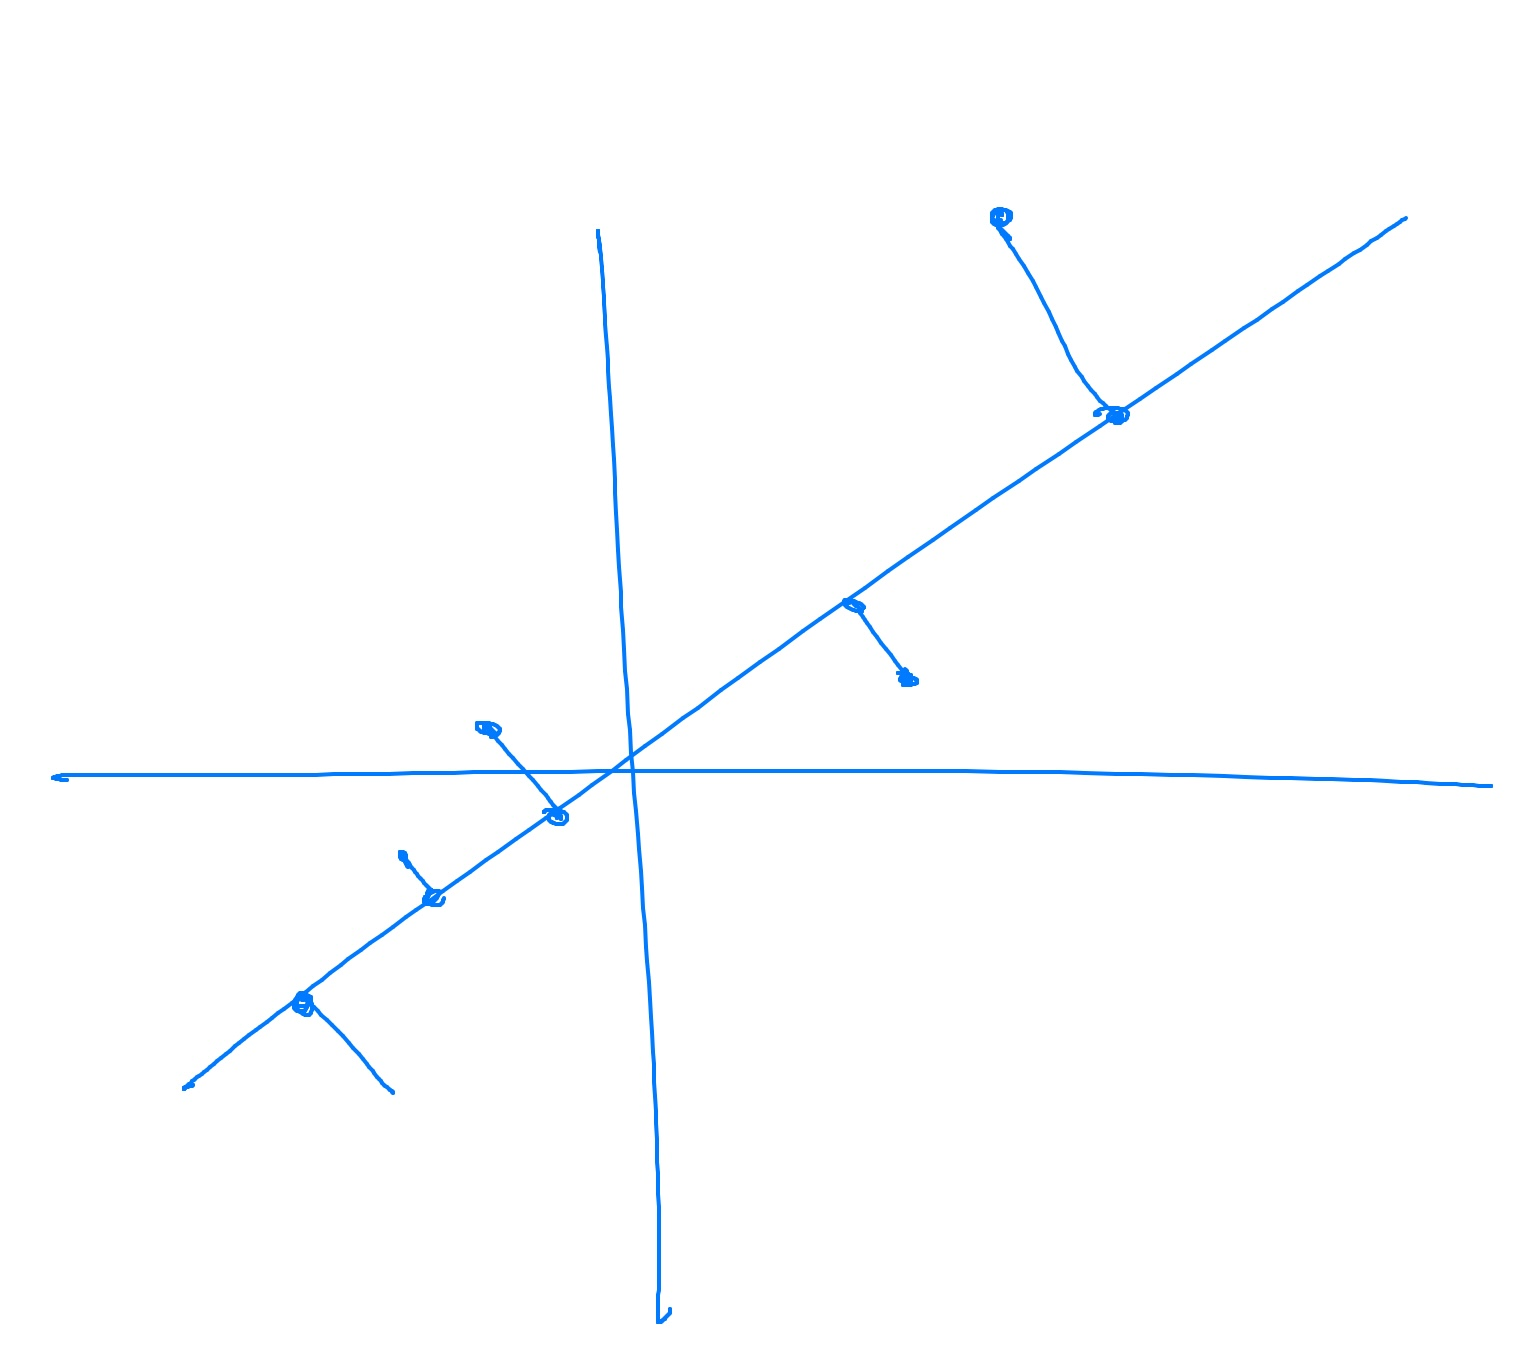
\includegraphics[width=8cm]{figs/PCA/PCA-proj.jpeg}
\caption{The projection operator $P$ embeds data to a lower dimensional subspace in $\R^d$}
\end{figure}

Note that in the sum in \eqref{eq:PCA-proj}, each eigenvector $v_i$ is multiplied by a coefficient $v_i^/T z$. We refer to these as the latent codes. In one to three dimensions, one may visualize these by treating them as coefficients of the canonical basis. This is illustrated in Figure \ref{fig:pca-latent-codes}. 
\begin{figure}[h] \label{fig:pca-latent-codes}
\centering
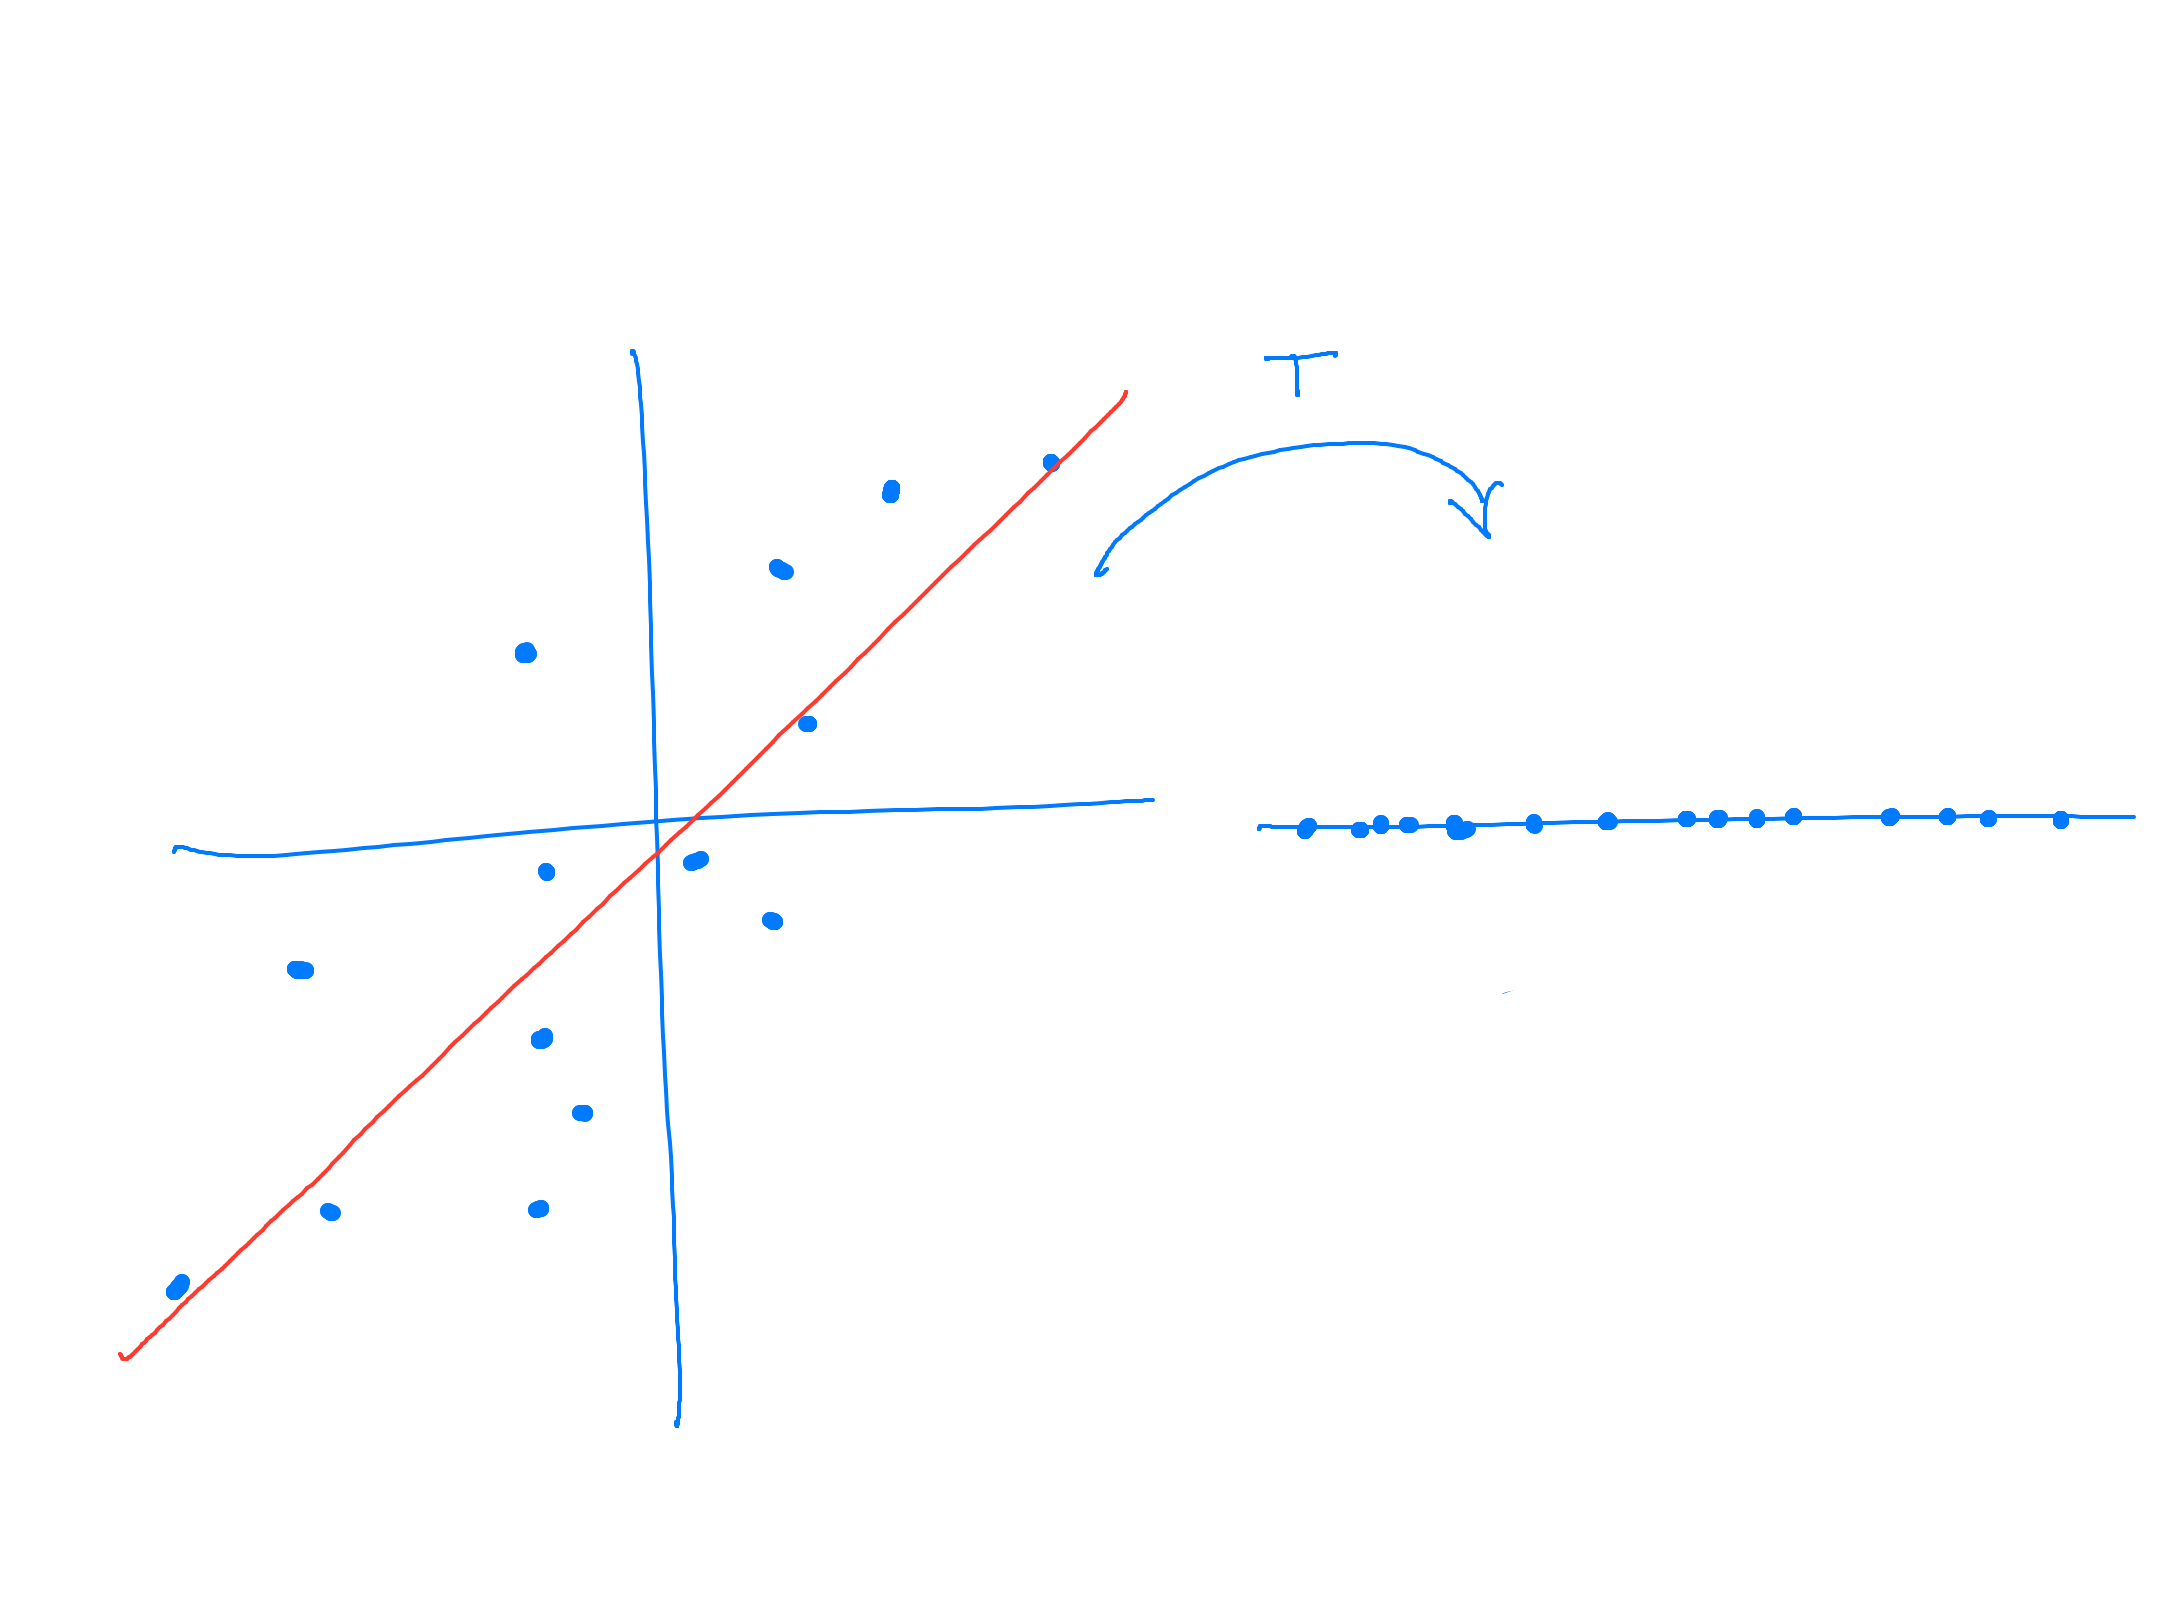
\includegraphics[width=10cm]{figs/PCA/PCA-latent-code.jpeg}
\caption{The projection operator $P$ embeds data to a lower dimensional subspace in $\R^d$.}
\end{figure}
Let
$$
T := 
\begin{pmatrix}
v_1^\T\\
\vdots\\
v_r^\T
\end{pmatrix}.
$$



\section{Examples}
TODO: Add Eigenfaces example. Note that this illustrates the "compression" aspect of PCA. Which is different from the dimensionality reduction. And it's kind of what the projection part is good for. 

\section{Unifying max variance and min reconstruction loss perspectives}
TODO: Ultimately, we're trying to optimize the same thing in both of these. Consider 2d example. One leg of a triangle is fixed between origin and data point. You have one degree of freedom to choose the other legs. You can maximize one leg, = maximizing variance. Or you can minimize another, which equates to minimizing reconstruction loss. See if this can be formalized a bit. 

\section{PCA and the Singular Value Decomposition}
IMPORTANT: In this section, I accidentally started using $X$ with $x_i$ as columns rather than rows. May not be consistent with rest of notes. Fix this. 

PCA reduces to computing the eigendecomposition of the sample covariance matrix $S = XX^\T$. In this section, we will see that this is equivalent to computing the SVD of $X$. 

\vspace{1em}
\noindent \textbf{SVD review:} For a possibly nonsquare matrix $A:\R^m\to\R^n$, the SVD involves computing a basis $(u_i)$ for the row and $(v_i)_i$ for the column space such that $Au_i = \sigma_i v_i$. Stick these basis vectors columnwise into matrics $U$ and $V$ so that $AU = V\Sigma $ or equivalently, $A = V\Sigma U^\T$, where $\Sigma$ has $(\sigma_i)$ on the diagonal. 
The singular values are computed by taking the eigendecomposition of $A^\T A$ and $A A^\T$. In particular, suppose that $(v_i)$ are an orthonormal set of eigenvectors of $AA^\T$ with eigenvalues $\sigma_i^2$ (exists by spectral theorem). Note that
$$
A A^\T v_i = \sigma_i^2 v_i \implies v_i^\T A A^\T v_i = \sigma_i^2 \|v_i\|^2 \implies \|Av_i\| = \sigma_i
$$
Let $u_i = \frac{1}{\sigma_i} A^\T v_i$, so that $u_i$ is unit norm. Note that
$$
AA^\T v_i = \sigma_i^2 v_i \iff A^\T A A^\T v_i = \sigma_i A v_i \iff A^\T A u_i = \sigma_i^2 u_i.
$$
Hence, $u_i$ is an eigenvector of $A^\T A$, and generally $(u_i)$ gives an orthonormal set of eigenvectors of $A^\T A$. 

\vspace{1em}
\noindent
\textbf{Back to PCA:} Returning to PCA, we see that computing the eigendecomposition of $XX^\T$ is equivalent to computing $V$ and $\Sigma$ in the SVD. 

In the SVD, one may retain only some of the singular vectors (is that what we call them) to obtain an optimal low-rank approximation to a matrix. This is summarized in the following result. 

\begin{theorem}[Ekhart-Mirsky-Young]
Let $A = V\Sigma U^\T$ and let $\Sigma_r = \myDiag(\sigma_1,\ldots, \sigma_r, 0,\ldots,0)$, where we use the convention that $\sigma_1\geq \sigma_2\geq \ldots$. Then $\hat A := V\Sigma_r U^\T$ is an optimal low rank approximation to $A$ in the senses that
$$
\|\hat A - A\|_F \leq \|B - A\|_F \mbox{ for all $B$ with rank $r$}
$$
and
$$
\|\hat A - A\|_2 \leq \|B - A\|_2 \mbox{ for all $B$ with rank $r$}.
$$
\end{theorem}
A note on proving this result: Proving the spectral norm component is easier. The Frobenius norm component requires (the approach I know of) using some tricks like Weyl's inequality. Both of these are nice exercises. 

\vspace{1em}
\textbf{Question}: How does this low-rank approximation perspective fit with PCA? 
The matrix of projected data points under PCA with $r$ principal components is given by 
$$
\tilde X = V_r V_r^\T X,
$$
where $V_r = (v_1,\ldots, v_r)$. On the other hand, the SVD low rank approximation of $X$ is given by
$$
\hat X = V \Sigma_r U^\T. 
$$
Note the former is simply a projection using the SVD basis vectors $V$ for the column space of $X$. The latter uses both basis vectors to map to singular value space, zero out unwanted components and then map back. Are these the same? 
To clarify this, let
$U_r\in \R^{d\times r}$ and $V_r \in \R^{m\times r}$, be matrices only retain the singular vectors corresponding to the $r$ largest singular values. Note that 
$$
\tilde X = V_r V_r^\T X = V_r V_r^\T V \Sigma U^\T = V_r [I_r, ~0] \Sigma U^\T = V_r \Sigma_r U_r^\T = V \Sigma_r U^\T = \hat X,
$$ 
where we have used the fact that V is constructed from an orthonormal basis. Hence, these are the same, and the projected data matrix $\tilde X$ in PCA is an optimal low-rank approximation to $X$. 
TODO: Clarify what each of these means. Double check the dimensions. Make sure everything works out. I don't want to be mapping from $\R^d$ to somewhere else, when mapping each column in $X$. 
Hence, despite the fact that PCA only computes $V$, it still allows us to construct an optimal low-rank approximation of $X$. 

\vspace{1em}
\noindent \textbf{High dimensional data}: An interesting follow on question from this is, what if $m \ll d$, i.e., data is very high-dimensional? If $d$ is large, then it may bay be expensive to compute the eigendecomposition of $S\in \R^{d\times d}$. But $U\in \R^{m\times m}$. Could we achieve the same results by computing $U$? The answer is yes, and follows readily from the SVD. Let $(u_i)$ be eigenvectors of $X^\T X\in \R^{m\times m}$. Note that this matrix doesn't have the same clean `covariance' interpretation (does it have a nice interpretation?). Let
$$
U_r = (u_1,\ldots, u_r)
$$
and let 
$$
\tilde X = XU_rU_r^\T.
$$
Applying the SVD to $X$ again, we see that this gives us the identical result to the standard PCA approach. It's interesting that here, the projection matrix is $\tilde X^\T = U_r U_r^\T X^\T$. We are now projecting rows of $X$ via the projection matrix $U_r U_r^\T$. Does this have a nice interpretation, like going to some nice subspace, like the minimum variance idea? 

\section{Kernel PCA}
In this section, we review Kernel PCA. I'm not exactly sure why people like Kernel PCA. 

TODO: Kernel PCA can follow as a really nice high-dimensional extension of PCA. But, I honestly don't get the point. I guess it's another way to visualize your data. But to what end? I haven't seen compelling examples visualizing, like, image datasets using kernel PCA. The most compelling example I can think of is that it's useful for better understanding kernel methods. Like, it lets you visualize a kernel method to some degree. What's I'm thinking is that I'm going to put a pin in this, and if I come back and study kernel methods, then I'll come back and flesh this section out. 

Plan: 
- The Bishop book as a clear exposition on deriving Kernel PCA that can basically be followed verbatim (I think... I actually only scanned that one)
- Two aspects of kernel PCA that intrigue me:
- Your data is mapped to a manifold. But when you project new data, you might actually not land on the manifold, so you can't go back to projected data. This idea seems interesting. 
- Examples with three concentric rings of data seem interesting. They can separate nicely with a linear separator. I'm still not entirely sure I understand the purpose of kernel PCA for this. Sure, it might help you to see clusters or something better. But nobody seems to know how to interpret it. 
- Honestly, if you really understood kernel PCA, could it be a powerful tool for really getting a good characterization of your data? Like, can you help people to interpret it better? Also, can you vary kernel parameters, like rbf bandwidth, to get a more complete characterization of your data topology?

%\section{Probabilistic PCA}
%
%\section{Autoencoders}
%
%\section{Variational Autoencoders}
